\documentclass{beamer}
%\documentclass[11pt, handout]{beamer}

\usepackage{graphicx}
\usepackage{xspace}
\usepackage{tikz}
\usepackage{circuitikz}
\usepackage{hyperref}
\usepackage{adjustbox} 
\usetikzlibrary{shapes.geometric, arrows}

\usepackage[backend=bibtex]{biblatex} 
\bibliography{thesis}
\renewcommand*{\bibfont}{\footnotesize}

%% Alex L's macros 
%% taken and co-opted from a variety of sources
%
%% generic commands
%\newcommand{\NN}{\mathbb{N}}
%\newcommand{\RR}{\mathbb{R}}
%\newcommand{\compindist}{\approx_C}
%
%% definition counter
%\newcounter{defcounter}
%\setcounter{defcounter}{0}
%\newenvironment{definition}{\medskip\noindent\refstepcounter{defcounter}{\bf Definition \thedefcounter}\hspace*{2pt}}{\hspace*{\fill}\nopagebreak[4]$\diamondsuit$\medskip}  
%
%% block quote
%\newenvironment{blockquote}{%
%  \par%
%  \medskip
%  \leftskip=4em\rightskip=2em%
%  \noindent\ignorespaces}{%
%  \par\medskip}
%
%% Author Macros -- colors: red, magenta, blue, orange
%\newcounter{al}
%\newcommand{\al}[1]{\textcolor{blue}{\{AL-\arabic{al}: #1\}}\addtocounter{al}{1}}
%\newcounter{cat}
%\newcommand{\cat}[1]{\textcolor{magenta}{\{CAT-\arabic{cat}: #1\}}\addtocounter{cat}{1}}
%\newcommand{\ignore}[1]{}
%
%% From CompGC paper
%%\renewcommand{\sim}{S}
%%\newcommand{\Input}{\ensuremath{\textsf{Input}}\xspace}
%%\newcommand{\Output}{\ensuremath{\textsf{Output}}\xspace}
%%\newcommand{\Inputs}{\ensuremath{\textsf{Inputs}}\xspace}
%%\newcommand{\Outputs}{\ensuremath{\textsf{Outputs}}\xspace}
%%\newcommand{\Components}{\ensuremath{\textsf{Components}}\xspace}
%
%\newcommand{\Gates}{\text{Gates}}
\newcommand{\C}{\sf {C}}
\newcommand{\GC}{\sf {GC}}
%\newcommand{\AllInputLabels}{\sf {AllInputLabels}}
%\newcommand{\InputLabels}{\sf {InputLabels}}
%\newcommand{\InputWires}{\text{InputWires}}
%\newcommand{\OutputWires}{\text{OutputWires}}
%\newcommand{\Wires}{\text{Wires}}
%\newcommand{\A}{\mathcal{A}}
%\newcommand{\OT}{\textsf{OT}} % or mathsf
\newcommand{\Enc}{\textsf{Enc}} % or mathsf
\newcommand{\Dec}{\textsf{Dec}}
\newcommand{\Gen}{\textsf{Gen}}
\newcommand{\EncInv}{\Enc^{-1}}
\newcommand{\EncDKC}{\textsf{EncDKC}}
\newcommand{\DecDKC}{\textsf{DecDKC}}
\newcommand{\EncDKCInv}{\EncDKC^{-1}}
%\newcommand{\compIndist}{\approx_D}
%\newcommand{\outputrv}{{\sf output}}
%\newcommand{\viewrv}{{\sf view}}
\newcommand{\CompGC}{\textsf{CompGC}\xspace}
%\newcommand{\JustGarble}{\textsf{JustGarble}\xspace}
%\newcommand{\Naive}{\textsf{Naive}\xspace}
%\newcommand{\scmc}{SCMC\xspace} % Single Communication Multiple Connnection


\renewcommand<>{\item}[1]{\only#2{\beameroriginal{\item}{#1}}}
    \mode<presentation> {
        \usetheme{default}
        \usecolortheme{seahorse}
        \setbeamertemplate{footline}[page number] 
        \setbeamertemplate{navigation symbols}{} 
    }

    % TODO: some sources, link to paper

    \title[Short title]{CompGC: Efficient Offline/Online Semi-honest Two-party Computation\\} 
    \author{Alex Ledger\\Arkady Yerukhimovich, Adam Groce, Alex Malozemoff} 
    %\institute[Reed College]{
    %    Reed College \\ 
    %}
    %\date{\today}
    \date{}

    \begin{document}

    \begin{frame}
        \titlepage 
    \end{frame}

    \begin{frame}
        \frametitle{Overview}
        \begin{enumerate}
            \item Two Party Secure Computation (2PC)
            \item Garbled Circuits
            \item Component-based Garbled Circuits
            \item Experiments and Results
        \end{enumerate}
    \end{frame}

    \begin{frame}
        \frametitle{The Millionaire Problem}
        \begin{itemize}
            \item Alice and Bob want to determine who is wealthier \cite{yao86}.
            \item They do not want to disclose their wealth to each other.
                \begin{itemize}
                    \item Alice has \$$x$, Bob has \$$y$.
                    \item Alice should not learn anything about $y$.
                    \item Bob should not learn anything about $x$.
                \end{itemize}
        \end{itemize}
        \begin{equation}
            f(x,y) = \left\{
                \begin{array}{ll}
                    Alice, & \quad y \leq x; \\
                    Bob, & \quad y > x.
                \end{array}
                \right.
            \end{equation}

            % http://www.alexirpan.com/2016/02/11/secure-computation.html
            \begin{figure}
                \centering
                \includegraphics[scale=0.8]{images/setup}
            \end{figure}
        \end{frame}

        \begin{frame}
            \frametitle{Security Properties}
            \begin{itemize}
                \item Confidentiality of Inputs
                    \begin{itemize}
                        \item Alice and Bob do not learn anything about the other's input.
                        \item Except for info that is inferable from their input and output.
                        \item Bob should not learn that $1,000,000 < x \leq 2,000,000$.
                        \item But if $y < x$ and $y = 2,000$, then he learns $x < 2,000$.
                    \end{itemize}
                \item Correctness
                    \begin{itemize}
                        \item Alice and Bob receive $f(x,y)$.
                    \end{itemize}
                \item Semi-honest
                    \begin{itemize}
                        \item We assume that each party obeys the protocol, but attemps to learn extra information from its interactions.
                    \end{itemize}
            \end{itemize}
        \end{frame}

        \begin{frame}
            \frametitle{Security}
            \begin{figure}
                \centering
                \includegraphics[scale=0.25]{images/security}
            \end{figure}
            A secure computation protocol is secure if Alice and Bob learn the same information in the real world as they would in ideal world.
        \end{frame}

        \begin{frame}
            \frametitle{Boolean Circuits}
            \begin{itemize}
                \item We encode a function $f$ into a circuit $C$.
                \item Circuit $C$ is made of AND, XOR and NOT gates.
                \item AND and XOR gates have two input wires and a single output wire
                \item A NOT gate has one input wire and one output wire
            \end{itemize}
            \begin{figure}
                \centering
                \includegraphics[scale=0.4]{images/and}
                \hfill
                \includegraphics[scale=0.4]{images/xor}
            \end{figure}
        \end{frame}

        \begin{frame}
            \frametitle{Boolean Circuits}
            \begin{itemize}
                \item Any function can be encoded into a circuit.
                \item Here is the less than circuit.
            \end{itemize}
            \begin{figure}
                \centering
                \includegraphics[scale=0.6]{images/less_than}
            \end{figure}
        \end{frame}

        %\begin{frame}
        %    \frametitle{Encryption}
        %    \center
        %    \includegraphics[scale=0.6]{images/encryption}
        %\end{frame}

        \begin{frame}
            \frametitle{Dual-key Encryption}
            \begin{itemize}
                \item Our protocol will use symmetric dual-key encryption.
                \begin{itemize}
                    \item Let $ct = \Enc_{k_0, k_1}(pt)$.
                    \item And $pt = \Dec_{k_0, k_1}(ct)$.
                    \item Can be instantiated with $\Enc_{k_0, k_1}(pt) = \Enc_{k_0}(\Enc_{k_1}(pt))$.
                \end{itemize}
                \item We also assume that you can tell if a decryption \textit{succeeds} or \textit{fails}.
            \end{itemize}
        \end{frame}

        \begin{frame}
            \frametitle{Oblivious Transfer (OT)}
            \begin{itemize}
                \item Alice potentially sends either $m_0$ or $m_1$ to Bob.
                \item Bob, without seeing $m_0$ or $m_1$, decides that he wants $m_b$.
                \item Bob receives $m_b$.
                \item Property 1: Alice does not know which message Bob recieved.
                \item Property 2: Bob doesn't anything about $m_{1-b}$.
            \end{itemize}

            \begin{figure}
                \includegraphics[scale=0.6]{images/ot}
            \end{figure}
        \end{frame}

        %\begin{frame}
        %    \frametitle{Hash Function in brief}
        %    \begin{itemize}
        %        \item Hash function $H: \{0,1\}^* \to \{0,1\}^{128}$
        %        \item For our purposes, $H$ maps any string to a uniform, random 128-bit string.
        %        \item A.k.a. $H$ is a random oracle.
        %    \end{itemize}
        %    \begin{figure}
        %        \center
        %        \includegraphics[scale=0.5]{images/hash}
        %    \end{figure}
        %    % sha-1 is actually a 160 bit hash function
        %\end{frame}

        \begin{frame}
            \frametitle{Roadmap of Garbled Circuits}
            \begin{enumerate}
                \item Alice (generator) \textit{garbles} the circuit.
                \item Alice sends the \textit{garbled tables} of each gate and some keys to Bob.
                \item Bob (evaluator) \textit{evaluates} the gate.
            \end{enumerate}

            \begin{figure}
                \includegraphics[scale=0.4]{images/high_level}
            \end{figure}
        \end{frame}

        \begin{frame}
            \frametitle{Garbling a Gate 1}
            Step 1. Alice assigns \textit{wire labels} to each wire.
            \begin{itemize}
                \item For each wire in the circuit, assign two random labels to each wire
                \item Wire $A$ has two wire labels $A_0$ and $A_1$.
                \item We say $A_0$ \textit{semantically represents} $0$, and $A_1$ \textit{semantically represents} $1$.
                \item And $A_0$ and $A_1$ are sampled uniformly at random from $\{0,1\}^k$.
            \end{itemize}

            \begin{figure}
                \centering
                \begin{circuitikz} \draw
                    (0,2) node[and port] (myand1) {}
                    (myand1.in 1) node[left=.8cm](a) {$A_0, A_1$}
                    (myand1.in 2) node[left=.8cm](b) {$B_0, B_1$}
                    (myand1.out) node[right=.25cm](c) {}
                    (myand1.out) node[right=.5cm](d) {$C_0, C_1$}
                    (a) -| (myand1.in 1)
                    (b) -| (myand1.in 2)
                    (myand1.out) -| (c)
                ;\end{circuitikz}
            \end{figure}
        \end{frame}

        \begin{frame}
            \frametitle{Garbling a Gate 2}
            Step 2. Alice constructs garbled table.
            \begin{itemize}
                \item Encrypt wire labels of $C$, $C_0$ and $C_1$, using the wire labels of $A$ and $B$.
                \item Randomly permute table
            \end{itemize}

            \begin{figure}
                \centering
                \begin{circuitikz} \draw
                    (0,2) node[and port] (myand1) {}
                    (myand1.in 1) node[left=.8cm](a) {$A_0, A_1$}
                    (myand1.in 2) node[left=.8cm](b) {$B_0, B_1$}
                    (myand1.out) node[right=.25cm](c) {}
                    (myand1.out) node[right=.5cm](d) {$C_0, C_1$}
                    (a) -| (myand1.in 1)
                    (b) -| (myand1.in 2)
                    (myand1.out) -| (c)
                ;\end{circuitikz}
            \end{figure}
            \begin{table}
                \centering
                \begin{tabular}{|c|c|c|}
                    \hline
                    $A$ & $B$ & Encryption \\
                    \hline
                    $A_0$ & $B_0$ & $\Enc_{A_0, B_0}(C_0)$ \\
                    $A_1$ & $B_0$ & $\Enc_{A_1, B_0}(C_0)$ \\
                    $A_0$ & $B_1$ & $\Enc_{A_0, B_1}(C_0)$ \\
                    $A_1$ & $B_1$ & $\Enc_{A_1, B_1}(C_1)$ \\                                               
                    \hline
                \end{tabular}
            \end{table}
        \end{frame}

        \begin{frame}
            \frametitle{Garbling a Gate 3}
            Step 3. Send garbled table to Bob.
            \begin{table}
                \centering
                \begin{tabular}{|c|}
                    \hline
                    $\Enc_{A_0, B_0}(C_0)$ \\
                    $\Enc_{A_1, B_0}(C_0)$ \\
                    $\Enc_{A_0, B_1}(C_0)$ \\
                    $\Enc_{A_1, B_1}(C_1)$ \\                                               
                    \hline
                \end{tabular}
            \end{table}
        \end{frame}

        \begin{frame}
            \frametitle{Garbling a Gate 4}
            Step 4. Alice sends input wire labels to Bob.
            \begin{itemize}
                \item Suppose $x \in \{0,1\}$ is Alice's input, and $y \in \{0,1\}$ is Bob's input.
                \item Alice sends $A_{x}$ to Bob.
                \item Alice sends $B_{y}$ to Bob via Oblivious Transfer
                    \begin{itemize}
                        \item The wire labels corresponding to her inputs.
                    \end{itemize}
                \item Bob has:
            \end{itemize}

            \begin{table}
                \begin{tabular}{|c|}
                    \hline
                    Garbled Table \\
                    \hline
                    $\Enc_{A_0, B_0}(C_0)$ \\
                    $\Enc_{A_1, B_0}(C_0)$ \\
                    $\Enc_{A_0, B_1}(C_0)$ \\
                    $\Enc_{A_1, B_1}(C_1)$ \\                                               
                    \hline
                \end{tabular}
                \qquad
                \begin{tabular}{|c|}
                    \hline
                    Input Labels \\
                    \hline
                    $A_x$ \\
                    $B_y$ \\
                    \hline
                \end{tabular}
            \end{table}
        \end{frame}

        \begin{frame}
            \frametitle{Garbling a Gate 5}
            Step 5. Bob evaluates the circuit
            \begin{itemize}
                \item Bob has the garbled table, $A_{x}$ and $B_{y}$.
                \item Bob trial decrypts each row of the garbled table, until an encrytion succeeds.
                \item Bob acquires $C_{x \wedge y}$.
                \item Bob has:
            \end{itemize}
            \begin{table}
                \begin{tabular}{|c|}
                    \hline
                    Garbled Table \\
                    \hline
                    $\Enc_{A_0, B_0}(C_0)$ \\
                    $\Enc_{A_1, B_0}(C_0)$ \\
                    $\Enc_{A_0, B_1}(C_0)$ \\
                    $\Enc_{A_1, B_1}(C_1)$ \\                                               
                    \hline
                \end{tabular}
                \qquad
                \begin{tabular}{|c|}
                    \hline
                    Input Labels \\
                    \hline
                    $A_x$ \\
                    $B_y$ \\
                    \hline
                \end{tabular}
                \qquad
                \begin{tabular}{|c|}
                    \hline
                    Output Label \\
                    \hline 
                    $C_{x \wedge y}$ \\
                    \hline
                \end{tabular}
            \end{table}

        \end{frame}

        \begin{frame}
            \frametitle{Garbling a Gate 6}
            Step 6. Bob gets a final answer.
            \begin{itemize}
                \item Alice sends $\Enc_{C_0}(0)$ and $\Enc_{C_1}(1)$ to Bob.
                \item Bob trial decrypts these with $C_{x \wedge y}$.
                \item One will succeed, and Bob will acquire $z = x \wedge y$.
                \item So Bob knows $z$, but not $x$!
            \end{itemize}

            \begin{table}
                \scriptsize
                \begin{tabular}{|c|}
                    \hline
                    Garbled Table \\
                    \hline
                    $\Enc_{A_0, B_0}(C_0)$ \\
                    $\Enc_{A_1, B_0}(C_0)$ \\
                    $\Enc_{A_0, B_1}(C_0)$ \\
                    $\Enc_{A_1, B_1}(C_1)$ \\                                               
                    \hline
                \end{tabular}
                \qquad
                \begin{tabular}{|c|}
                    \hline
                    Input Labels \\
                    \hline
                    $A_x$ \\
                    $B_y$ \\
                    \hline
                \end{tabular}
                \qquad
                \begin{tabular}{|c|}
                    \hline
                    Output Label \\
                    \hline 
                    $C_{x \wedge y}$ \\
                    \hline
                \end{tabular}
                \qquad
                \begin{tabular}{|c|}
                    \hline
                    Output Map \\
                    \hline 
                    $\Enc_{C_0}(0)$ \\
                    $\Enc_{C_1}(1)$ \\
                    \hline
                \end{tabular}
            \end{table}
        \end{frame}

        \begin{frame}
            \frametitle{Security Considerations}
            \begin{itemize}
                \item Think about what Alice acquires:
                    \begin{itemize}
                        \item Alice generates objects and sends them to Bob
                        \item So she doesn't have many opportunities to learn about Bob's input.
                        \item The only place she can learn anything is during OT.
                    \end{itemize}
                \item Think about what Bob acquires:
                    \begin{enumerate}
                        \item Garbled table
                        \item Input wire labels: $A_a$ and $B_b$
                        \item Encryptions of output: $\Enc_{C_0}(0)$ and $\Enc_{C_1}(1)$
                    \end{enumerate}
                \item Can Bob learn anything about $x$?
                    \begin{itemize}
                        \item If he could decrypt another row of the garbled table, then we would learn something.
                        \item But he can't, because he doesn't have the keys.
                        \item So he doesn't learn anything because everything is encrypted and he doesn't have keys to decrypt anything else.
                    \end{itemize}
            \end{itemize}
            \begin{figure}
                \center
                \includegraphics[scale=0.15]{images/security}
            \end{figure}
        \end{frame}

        \begin{frame}
            \frametitle{Extending a garbled gate into a garbled circuit}
            \begin{itemize}
                \item To operate on a more complex function, the operation is recursed.
                \item The output wires of the first gates are used as inputs to subsequent gates.
                \item Alice only sends output maps for the final gates.
            \end{itemize}
            \begin{figure}
                \includegraphics[scale=0.6]{images/less_than}
                %\includegraphics[scale=0.4]{images/high_level}
            \end{figure}
        \end{frame}

        \begin{frame}
            \frametitle{The Garbled Circuit Protocol}
            \begin{figure}
                \includegraphics[scale=0.8]{images/high_level}
            \end{figure}
        \end{frame}
        \begin{frame}
            \frametitle{The cost of garbled circuits}
            \begin{itemize}
                \item Alice sends $4$ ciphertexts per gate, since the garbled table has $4$ rows, to Bob.
                \item Based on empirical work, bandwidth is the biggest bottleneck in garbled circuits.
                \item So reducing the size of the garbled table is of utmost priority.
            \end{itemize}

            \begin{figure}
                \includegraphics[scale=0.6]{images/less_than}
                %\includegraphics[scale=0.4]{images/high_level}
            \end{figure}
        \end{frame}

        \begin{frame}
            \frametitle{Reducing the size of the garbled table with Free XOR}
            \begin{itemize}
                    \small
                \item Let $\Delta \gets \{0,1\}^n$ be fixed globally in a circuit \cite{freexor}.
                \item For each input wire $A$, sample a single ciphertext; call it $A$.
                    \begin{itemize}
                            \footnotesize
                        \item The \textit{zeroith} wire label is $A$.
                        \item The \textit{first} wire label is $A \oplus \Delta$.
                    \end{itemize}
                \item Set output wire $C$ of a gate to be $A \oplus B$ (the xor of its input wires).
                \item Bob \textit{evaluates} an XOR gate by XORing the two input labels.
                    \begin{align*}
                        (A \oplus a\Delta) \oplus (B \oplus b\Delta) = A \oplus B \oplus (a \oplus b)\Delta
                    \end{align*}
                \item So XOR gates do not require a garbled table, aka they're free.
            \end{itemize}
        \end{frame}

        \begin{frame}
            \frametitle{Offline/Online}
            \small
            \begin{itemize}
                \item Imagine two banks use secure computation during their daily operations.
                \item At night - the offline phase - they exchange garbled circuits (the garbled tables)
                \item During the day - the online phase - they exchange input wire labels and evaluate the pre-exchanged garbled circuits.
                \item The computation is fast!
                \item Problems:
                    \begin{itemize}
                            \footnotesize
                        \item Functions are decided at night - no room for flexibility
                        \item Input size is fixed at night 
                    \end{itemize}
            \end{itemize}

            \begin{figure}
                \scalebox{0.75}{
                    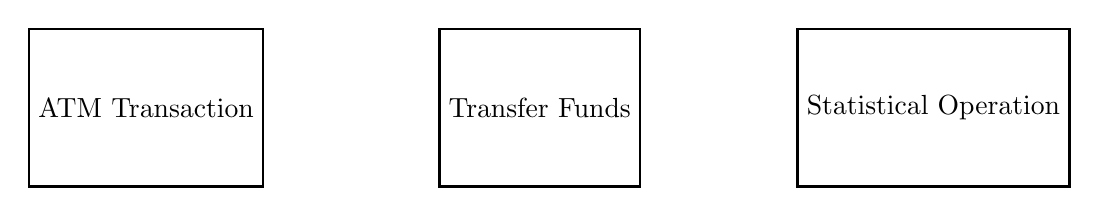
\begin{tikzpicture}
                        [
                            square/.style = {draw, shape=rectangle, minimum height=2cm, minimum width=2cm, node distance=2cm, line width=1pt},
                            empty/.style = {draw, shape=rectangle, minimum height=2cm, minimum width=2cm, node distance=2cm, line width=1pt, draw=white},
                        ]

                        \node[square] (0c) at (0,0)      {ATM Transaction};
                        \node[square] (1c) at (5cm,0)    {Transfer Funds};
                        \node[square] (2c) at (10cm,0)   {Statistical Operation};
                    \end{tikzpicture}
                }
            \end{figure}
        \end{frame}

        \begin{frame}
            \frametitle{Component-based Garbled Circuits}
            \begin{itemize}
                \item Goal: Add flexibility to offline/online garbled circuits \cite{compgc}.
                \item Key observation: many useful functions in the real world are composed of small, standard components.
                    \begin{itemize}
                        \item E.g. addition, subtraction, matrix operations
                        \item Leveshtein distance algorithm - a dynamic algorithm
                        \item Encryption is a common component
                    \end{itemize}
                \item Idea: chain garbled circuits together
                    \begin{itemize}
                        \item Take the output of one garbled circuit and plug it into another garbled circuit
                    \end{itemize}
            \end{itemize}
            \begin{figure}
                \scalebox{0.75}{
                    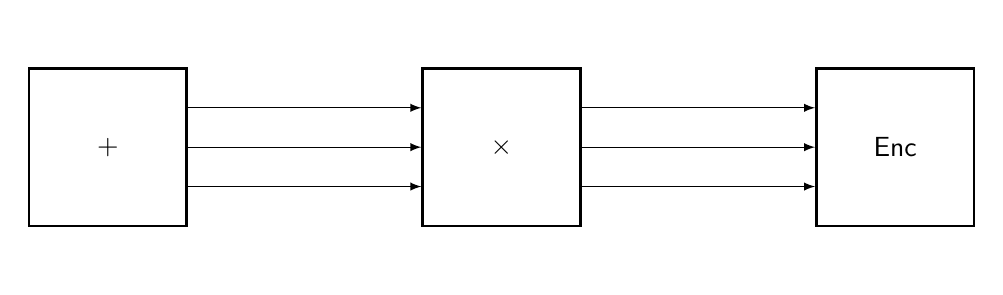
\begin{tikzpicture}
                        [
                            square/.style = {draw, shape=rectangle, minimum height=2cm, minimum width=2cm, node distance=2cm, line width=1pt},
                            empty/.style = {draw, shape=rectangle, minimum height=2cm, minimum width=2cm, node distance=2cm, line width=1pt, draw=white},
                        ]

                        \node[empty] (0a) at (0,0.5)     {};
                        \node[empty] (0b) at (0,-0.5)     {};
                        \node[square] (0c) at (0,0)     {$+$};

                        \node[empty] (1a) at (5cm,0.5)   {};
                        \node[empty] (1b) at (5cm,-0.5)   {};
                        \node[square] (1c) at (5cm,0)   {$\times$};

                        \node[empty] (2a) at (10cm,0.5)   {};
                        \node[empty] (2b) at (10cm,-0.5)   {};
                        \node[square] (2c) at (10cm,0)   {$\Enc$};

                        \draw [-latex] (0a.east) -- (1a.west);
                        \draw [-latex] (0b.east) -- (1b.west);
                        \draw [-latex] (0c.east) -- (1c.west);

                        \draw [-latex] (1a.east) -- (2a.west);
                        \draw [-latex] (1b.east) -- (2b.west);
                        \draw [-latex] (1c.east) -- (2c.west);

                    \end{tikzpicture}
                }
            \end{figure}

        \end{frame}

        \begin{frame}
            \frametitle{How to chain garbled circuits}
            \begin{itemize}
                \item Suppose that we are chaining a garbled circuit with output wire $A$ to garbled circuit with input wire $X$.
                \item We want $A \to X$ and $A \oplus \Delta \to X \oplus \Delta$.
                \item Straightforward:
                    \begin{itemize}
                        \item Alice sends Bob {\color{blue}$L_{AX}$}$ = A \oplus X$
                        \item Bob sets $X_* \gets A_* \oplus$ {\color{blue}$L_{AX}$}
                    \end{itemize}
                    \begin{figure}
                        \scalebox{0.75}{
                            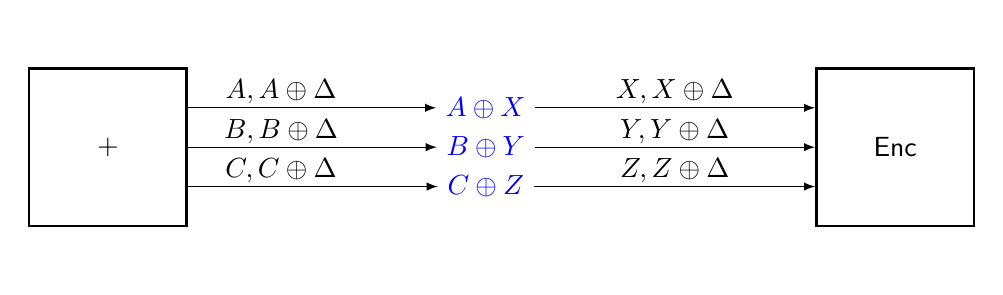
\begin{tikzpicture}
                                [
                                    square/.style = {draw, shape=rectangle, minimum height=2cm, minimum width=2cm, node distance=2cm, line width=1pt},
                                    empty/.style = {draw, shape=rectangle, minimum height=2cm, minimum width=2cm, node distance=2cm, line width=1pt, draw=white},
                                ]

                                \node[empty] (0a) at (0,0.5)     {};
                                \node[empty] (0b) at (0,-0.5)     {};
                                \node[square] (0c) at (0,0)     {$+$};

                                \node[color=blue] (mida) at (4.8cm,0.5)   {$A \oplus X$};
                                \node[color=blue] (midb) at (4.8cm,-0.5)  {$C \oplus Z$}; 
                                \node[color=blue] (midc) at (4.8cm,0)     {$B \oplus Y$};

                                \node[empty] (1a) at (10cm,0.5)   {};
                                \node[empty] (1b) at (10cm,-0.5)   {};
                                \node[square] (1c) at (10cm,0)   {$\Enc$};

                                \node (x0) at (2.2cm,0.7) {$A, A \oplus \Delta$};
                                \node (y0) at (2.2cm,-0.3) {$C, C \oplus \Delta$};
                                \node (z0) at (2.2cm,0.2) {$B, B \oplus \Delta$};

                                \node (x1) at (7.2cm,0.7) {$X, X \oplus \Delta$};
                                \node (y1) at (7.2cm,-0.3) {$Z, Z \oplus \Delta$};
                                \node (z1) at (7.2cm,0.2) {$Y, Y \oplus \Delta$};

                                \draw [-latex] (0a.east) -- (mida.west);
                                \draw [-latex] (0b.east) -- (midb.west);
                                \draw [-latex] (0c.east) -- (midc.west);

                                \draw [-latex] (mida.east) -- (1a.west);
                                \draw [-latex] (midb.east) -- (1b.west);
                                \draw [-latex] (midc.east) -- (1c.west);
                            \end{tikzpicture}
                        }
                    \end{figure}
            \end{itemize}
        \end{frame}

        \begin{frame}
            \frametitle{AES with 10 Components}
            \centering
            \includegraphics[scale=0.34]{images/aes_rounds}
            \pause
            \\
            Are component-based garbled circuits secure?
        \end{frame}

        \begin{frame}
            \frametitle{Setup for Our Experiments}
            \begin{itemize}
                \item Offline phase:
                    \begin{enumerate}
                        \item Generator generates, garbles and sends component-circuits to evaluator.
                        \item Generator and evaluator complete OT preprocessing
                    \end{enumerate}
                \item Online phase:
                    \begin{enumerate}
                        \item Generator sends wire labels for their inputs
                        \item Generator and garbler complete OT
                        \item Generator sends link labels
                        \item Evaluator links and evaluates components
                    \end{enumerate}
            \end{itemize}
        \end{frame}

        \begin{frame}
            \frametitle{General Experiments}
            \begin{itemize}
                \item AES: 10 AES Rounds
                \item CBC: 100 AES Rounds and 10 XOR for 10-block CBC
                \item Levenshtein 30: 900 Levenshtein Components
                \item Levenshtein 60: 3600 Levenshtein Components
            \end{itemize}
        \end{frame}

        \begin{frame}
            \frametitle{AES with 10 Components}
            \centering
            \includegraphics[scale=0.34]{images/aes_rounds}
        \end{frame}

        \begin{frame}
            \frametitle{Leveshtein Component}
            \centering
            \includegraphics[scale=0.3]{images/LevenCirc}
            \\
            Figure from \cite{faster2pc}
        \end{frame}

        \begin{frame}
            \frametitle{General Results}
            \centering
            \includegraphics[scale=0.3]{images/results}
            \begin{itemize}
            \footnotesize
                \item Times in milliseconds. Communication in Megabits.
                \item Naive is normal garbled circuits with optimizations and preprocessed OT.
                \item Times are over network with 50Mbit/s bandwidth and 20ms latency
                \item All timings are online time of evaluator averaged over 100 trials.
                \item Experiments done on a laptop.
            \end{itemize}
        \end{frame}

        \begin{frame}
            \frametitle{Machine Learning Experiments}
            \begin{itemize}
                \item Private classification: Suppose that a machine learning model exists, and a party wants to privately classify their data with the model.
                \item We implement functions to query ML models using basic components \cite{bost}:
                % TODO: pointed out by Bost et al.
                    \begin{itemize}
                        \item Less than
                        \item Inner product
                        \item Argmax
                        \item Addition
                        \item Select
                    \end{itemize}
                \item ML classifications:
                    \begin{itemize}
                        \item Decision Tree
                        \item Naive Bayes
                        \item Linear (Hyperplane) Classification
                    \end{itemize}
                \item We use real data UCI Machine Learning repository \cite{uci}.
            \end{itemize}
        \end{frame}

        \begin{frame}
            \frametitle{Decision Tree Node}
            \centering
            \includegraphics[width=0.5\textwidth]{images/tree}
            \includegraphics[width=0.5\textwidth]{images/decision_tree_node}
            \\
            \footnotesize
            Figure on left from \cite{bost}
        \end{frame}

        \begin{frame}
            \frametitle{Naive Bayes}
            \centering
            \includegraphics[scale=0.25]{images/Naive_Bayes}
            \begin{itemize}
                \item Select$(arr, idx) \to arr[idx]$.
                \item Add$(x, y) \to x + y$.
                \item Argmax$(a, b, c, ...) \to$ index of largest of input.
            \end{itemize}
        \end{frame}

        \begin{frame}
            \frametitle{Linear Classifier}
            \centering
            \includegraphics[scale=0.25]{images/linear_classifier}
        \end{frame}

        \begin{frame}
            \frametitle{Bigger Linear Classifier}
            \centering
            \includegraphics[scale=0.25]{images/bigger_linear_classifier}
        \end{frame}

        \begin{frame}
            \frametitle{Results}
            \begin{itemize}
                \item Times in milliseconds. Communication in Megabits.
                \item Naive is normal garbled circuits with optimizations and preprocessed OT.
                \item Times in parentheses are over network with bounded bandwidth: 50Mbit/s bandwidth and 20ms latency
                \item All timings are online time of evaluator averaged over 100 trials.
                \item Rnds is the number of roundtrips between parties.
            \end{itemize}

        \end{frame}

        \begin{frame}
            \frametitle{Results}
            \centering
            \includegraphics[scale=0.25]{images/ml_results}
        \end{frame}

        \begin{frame}
            \frametitle{Conclusion}
            \begin{itemize}
                \item Communicating the garbled circuit is the bottleneck the garbled circuit protocol.
                \item Many functions can be constructed from a small set of components.
                \item Component-based garbled circuits substantially reduce bandwidth and improve online running time over standard garbled circuits.
            \end{itemize}
        \end{frame}

        \begin{frame}
            \frametitle{Bibliography}
            \printbibliography
        \end{frame}

        \end{document} 
